%! TeX root = ../main.tex
\section{Обзор методов оценки угла прихода}


\subsection{Характеристики канала связи миллиметровых длин волн}
Миллиметровая модель канала имеет ряд особенностей, которые описаны во множестве
литературных источников и мировых стандартах \cite{Maltsev2010, Maltsev2017,
    Xu2002, Akdeniz2014, Rappaport2015}. Основные особенности следующие:
\begin{itemize}
    \item Малое влияние дифракции
    \item Высокие потери в канале связи
    \item Потери на шероховатостях отражающих поверхностей
    \item Пути распространения могут быть ассоциированы с геометрическими лучами
\end{itemize}

Последний пункт является наиболее важным с точки зрения алгоритмов оценки угла прихода волны 
(Angle of Arrival).
Также, из этого свойства канала следует, что количество различимых сильных путей
распространения относительно невелико. Это подтверждено результатами
измерений каналов как для внутренних, так и для наружных сценариев.

Например, результаты измерения AOA в помещении представлены на рис.
\ref{fig:3.1}.  На рис. \ref{fig:3.2} представлены уникальные AOA в случае
уличного сценария <<Манхеттен>>. Можно заметить, что среднее число хорошо
различимых независимых путей распространения $\mu=4.7$, что достаточно
мало.



\begin{figure}[ht!]
    \centering
    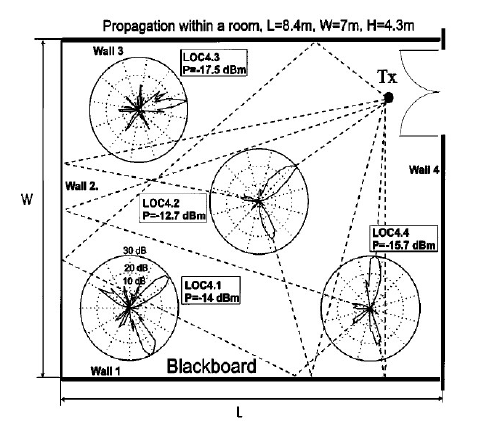
\includegraphics[width=0.6\linewidth]{figs/fig3.1}
    \caption{ Измерение AOA для определения пути распространения в помещении,
        измеренная мощность показана в полярных координатах, $P$ -- максимум
        измеренной мощности. Геометрические лучи показаны только для позиций
        4.2 и 4.4 \cite{Xu2002}.}
    \label{fig:3.1}
\end{figure}

\begin{figure}[ht!]
    \centering
    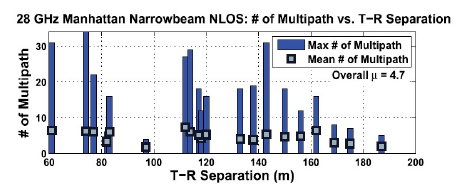
\includegraphics[width=0.8\linewidth]{figs/fig3.2}
    \caption{
        Зависимость числа различимых путей распространения для различных углов азимута и элевации от расстояния между источником и приемником.
        Среднее значение по всем измерениям составило $\mu=4.7$. Измерения проводились с узкой диаграммой направленности в Махеттене \cite{Rappaport2015}.}
    \label{fig:3.2}
\end{figure}

На основе рассмотренных работ, можно сделать вывод, что в данной модели
канала чаще всего можно выделить несколько сильнейших путей
распространения и определить их AOA.

\subsection{Обзор некоторых методов оценки угловой координаты источника излучения}
\label{sec:review}

Канал в миллиметровом диапазоне можно представить в виде
набора геометрических лучей.  Самые сильные лучи могут быть
использованы для передачи данных. Как правило, диаграмма направленности
антенны формируется по направлению луча прямой видимости (Line of Sight).
Однако в случае не прямой видимости (Non Line of Sight), может быть
выбран самый сильный отраженный геометрический луч. 

Оценка угла прихода, часто рассматривается в задачах
радиолокации.  Для этих задач  давно разработаны алгоритмы и аппаратные реализации
ещё во времена зарождения радиолокации. Эти алгоритмы совершенствовались с
появлением фазированных антенных решеток.  
Этот может оказаться очень  полезным c учетом  аппаратных ограничений систем
связи 5G NR -- число цифровых портов обычно мало по сравнению с имеющимся
количеством элементов антенной решетки. 

Другой набор алгоритмов пришел из задач спектрального анализа.  В них обычно
предполагается, что сигнал каждой антенны принимается независимо.  Эти алгоритмы
очень эффективны и дают возможность оценить направления на несколько целей
(лучей) одновременно и имеют сверхразрешающую способность, но c другой стороны,
они требуют значительных вычислительных ресурсов.  

В этом разделе мы рассмотрим и систематизируем существующие подходы к оценке
АОА, которые нам удалось найти в открытых литературных источниках.  Будут
представлены их преимущества и недостатки.  На этапе моделирования в следующей
части этой работы, мы сократим этот список и выделим наиболее перспективные
методы.

\subsubsection{Методы Фурье и Бартлетта}
\label{sec:3.2.1} \label{sec:Fourier}

Простейшая алгоритм оценки AOA в зарубежной литературе называется бимформингом \cite{Tuncer2009, Stoica2005} или методом Фурье \cite{Allen2006}.
Основная идея заключается в максимизации мощности, принятой с определенного
направления.

Обозначим сигнал $\vec{y}(t)$ принятой антенной решеткой от некоторого
удаленного источника
\begin{equation}
    \label{eq:3.1}
    \vec{y}(t) = a(t) \vec{s}(\phi_{src}) + \vec{\xi}(t),
\end{equation}
где ${\vec{s}(\phi_{src})}$ -- фазирующий вектор,
$\phi_{src}$ -- угол прихода (AOA); $\vec \xi$ -- вектор шума.
Каждый элемент фазирующего вектора представляется в виде
\begin{equation}
    \label{eq:3.2}
    \qty{\vec{s}(\phi)}_n = \exp{-i(\vec k (\phi), \vec \rho_n)},
\end{equation}
где $\vec k (\phi_{src})$ -- волновой вектор плоской волны, $\vec\rho_n$ радиус-вектор
$n$-го элемента антенны.
В случае эквидистантной антенной решетки, последнее уравнение приведется
к виду
\begin{equation}
    \qty{\vec s(\phi)}_n = \exp{i2\pi\frac{d}{\lambda}\sin(\phi)n},
\end{equation}
где $d$ -- расстояние между элементами антенной решетки, $\lambda$ -- длина
волны излученного сигнала.

Чтобы получить максимальную мощность с некоторого направления $\phi$ необходимо
сформировать соответствующую диаграмму направленности с помощью
весового вектора антенной решетки $\vec w (\phi) = \vec s(\phi)/\rVert(\vec
    s(\phi))\lVert$.  Тогда, можно найти мощность излученного с АР сигнала.
\begin{equation}
    p(\phi) = \abs{\vec w^H (\phi) \vec y}^2.
\end{equation}

Оценкой AOA будет являться значение аргумента $\phi$, обеспечивающего максимум функции $p(\phi)$
\begin{equation}
    \phi^* = \arg\max p(\phi)
\end{equation}

\begin{figure}[ht!]
    \centering
    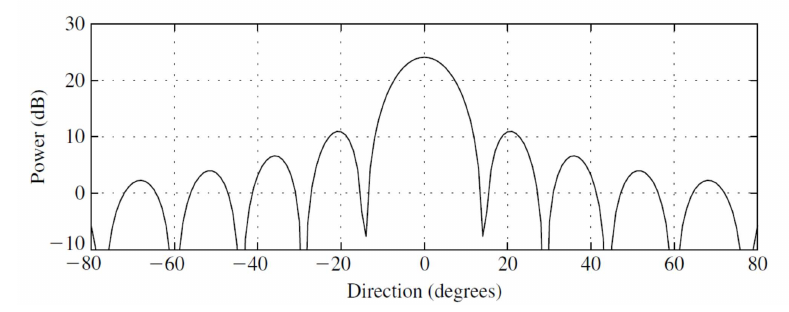
\includegraphics[width=\linewidth]{figs/fig3.9}
    \caption{ДН для 16-ти элементной эквидистантной линейной
        решетки ($\frac{d}{\lambda}=0.5$), сформированной в направлении $0^\circ$
        \cite{Tuncer2009}. }
    \label{fig:3.9}
\end{figure}

Для фазированной антенной решетки поиск $\phi^*$ может быть реализован во временной
области с помощью сканирования диаграммой направленности. Если количество
приемников (цифровых портов) равно количеству антенных элементов, искомая
функция $p(\phi)$ может быть оценена в цифровой области \cite{Stoica2005}.  В
литературе этот подход также называется методом Бартлетта \cite{Godara2004}.

Функция $p(\phi)$ примет вид
\begin{equation}
    p(\phi) = \frac{\vec s^H(\varphi) \hat{\vec M} \vec s (\phi)}{N^2},
\end{equation}
где $\hat{\vec M}$ -- оценка корреляционной матрицы принятого сигнала
\begin{equation}
    \label{eq:3.7}
    \hat{\vec M} = \frac{1}{L} \sum\limits_{t=1}^{L} \vec y(t) y^H (t)
\end{equation}

\paragraph{Преимущества}%
\begin{enumerate}
    \item Теоретически, метод Фурье и метод Бартлетта являются оптимальными
          решениями для оценки AOA в случае однолучевого канала.
    \item Легко технически реализуется на конечном устройстве и требует мало
          вычислительных мощностей.
\end{enumerate}

\paragraph{Недостатки}%

\begin{enumerate}
    \item На практике, точность поиска снижается.
          Это происходит, во-первых,  потому что производная функции $p(\phi)$
          в направлении на максимум равна нулю и из-за <<плоской>> вершины сложно
          точно определить точку экстремума. Во-вторых, необходимо
          обеспечить высокую дискретизацию по углу для обеспечения приемлемой
          оценки.
    \item Алгоритм может не подойти в случае быстро движущихся пользователей, если поиск реализован с помощью сканирования во временной области.
    \item Метод обеспечивает разрешающую способность, зависящую
          от ширина главного лепестка ДН. Увеличение отношения сигнал/шум (ОСШ) или времени
          сканирования не приведет к качественному улучшению разрешения.  Это делает
          этот подход малопригодным для оценки многолучевого АОА.
    \item В случае нескольких близко расположенных АОА присутствует
          значительная систематическая ошибка.
\end{enumerate}


\subsubsection{Метод максимального правдоподобия}%
\label{sub:metod_maksimal_nogo_pravdopodobiia}
\label{sec:MLE-algorithm}
При наличии нескольких путей распространения, оптимальная оценка AOA может быть
получена с помощью максимально правдоподобной оценки (Maximum Likelihood
Estimator) \cite{Tuncer2009}.  

Рассмотрим модель сигнала:
\begin{equation}
    \label{eq:3.8}
    \vec y(t) = \sum\limits_{q=1}^{J} a_q(t)\vec s(\phi_q) + \vec \xi(t),
\end{equation}
где $J$ число путей распространения; $a_q(t)$ -- комплексная амплитуда $q$-то
луча, $\vec s(\phi_q)$ -- фазирующий вектор;  $\phi_q$ -- угол прихода (AOA) $q$-то
луча и $\xi(t)$ -- вектор белого гауссового шума.

Для этой модели канала критерий МП может быть записан как критерий минимума
среднеквадратичной ошибки (Minimum Mean Square Error)
\begin{equation}
    d(\phi_1, \hdots, \phi_J) = \sum\limits_{t}^{} \abs{\vec(t) -
        \sum\limits_{q=1}^{J} a_q(t) \vec s(\phi_q)}^2 \to \min_{\phi_q}.
\end{equation}
Что можно переписать в виде
\begin{equation}
    \label{eq:3.10}
    d(\phi_1, \hdots, \phi_J) = \sum\limits_{t}^{} \vec y^H(t) \vec
    P_\perp(\phi_1, \hdots, \phi_J) \vec y(t) \to \min_{\phi_q},
\end{equation}
\begin{equation}
    \vec P_\perp(\phi_1, \hdots, \phi_J) = \vec E - \vec S(\vec S^H \vec S)^{-1}
    \vec S^H,
\end{equation}
где $\vec P_\perp$ -- проекционная матрица, 
$\vec S = \qty[\vec s(\phi_1) \dots \vec s (\phi_J)]$. 

Минимизация $d(\phi_1, \hdots, \phi_J)$ в общем случае производится численно и
как правило требует больших вычислительных ресурсов для реализации $J$-мерной
минимизации \cite{Tuncer2009}. 


\paragraph{Преимущества}%
\begin{enumerate}
    \item Обеспечивает оптимальное решение в случае нескольких сильных путей распространения 
\end{enumerate}

\paragraph{Недостатки}%
\begin{enumerate}
    \item Требует большого количества цифровых портов 
    \item Требует больших вычислительных затрат
    \item Не позволяет оценить количество доминирующих путей распространения. Если их количество неизвестно, метод становится неоптимальным. 
\end{enumerate}

\subsubsection{Метод моноимпульса}%
\label{sec:monopulse}

Данная разновидность формирования ДН часто называется моноимпульсом и обычно 
используется в радиолокационных системах для задач слежения. 
Этот алгоритм использует разницу между мощностью двух измеренных лучей как метрику для 
оценки AOA \cite{Tuncer2009}. Вводится следующая функция 
\begin{equation}
    \label{eq:3.11}
    b(\phi) = \frac{1}{\Delta} \qty(\abs{\vec w^H(\phi+0.5 \Delta)\vec y}^2)
    -
    \qty(\abs{\vec w^H(\phi-0.5 \Delta)\vec y}^2) \approx \dv{p(\phi)}{\phi} ,
\end{equation}
где $p(\phi)$ и $\vec w(\phi)$ были определены в разделе \ref{sec:3.2.1}, $\Delta$ -- некоторый скаляр. Тогда, оценка AOA
заключается в поиске такого угла $\phi$, который обеспечивает нуль функции $b(\phi)$
\begin{equation}
    \label{eq:3.12}
    \phi = \arg\qty{b(\phi) = 0}.
\end{equation}

Величина $\Delta$ может быть порядка ширины луча, но  $b(\phi)$ всё равно будет
хорошо аппроксимироваться производной $p(\phi)$, поскольку $b(\phi)$ почти
линейна в большом диапазоне углов около нуля \cite{Tuncer2009}.  

\begin{figure}[ht]
    \centering
    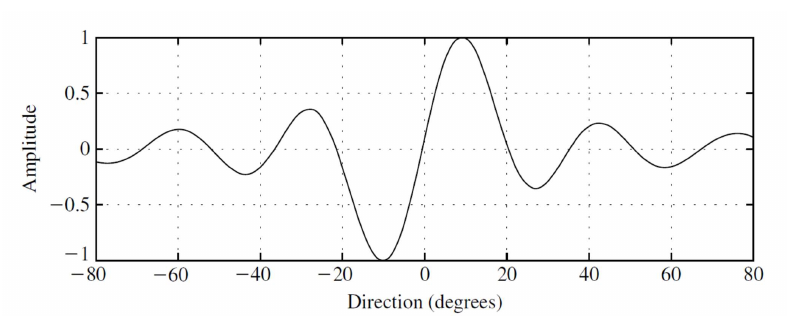
\includegraphics[width=\linewidth]{figs/fig3.11}
    \caption{Зависимость метрики $b(\phi)$ для 16-ти элементной ULA \cite{Tuncer2009}. Направление на источник -- 0 град.}
    \label{fig:3.11}
\end{figure}
% Another variant of the algorithm is often called Monopulse Ratio or Amplitude
% Comparison Monopulse \cite{Mosca1969}. This algorithm requires coherent reception with two
% channels (RF-chains): sum and difference. The sum channel is formed with beam
% pattern which has a maximum for a certain direction. The difference beam
% pattern has a null for this direction. In \cite{Kim2018} the algorithm which uses TDM for
% sum and difference channels is proposed and investigated. It employs cycle
% prefix of OFDM signal to receive two identical signals with different beam
% patterns using a single RF-chain and phased antenna array. This approach seems
% promising, but there are some issues related to phase shifter switching delay
% and multipath propagation influence.
% The metric of monopulse ratio is \cite{Kim2018}
% \begin{equation}
%     \label{eq:}
%     \tan(\frac{N}{4}(\phi_{src} - \phi)) =
%     \frac{Im\qty{\sum\limits_{k} y_d(k) y_s^*(k)}}{\sum\limits_{k}
%         \abs{y_s(k)}^2},
% \end{equation}
% where $\phi_{src}$ is actual  AOA;  $\phi$ is roughly estimated AOA via beam
% sweeping (it is the direction of the sum beam); N is number of antenna
% elements; $y_s(k)$ and  $y_d(k)$ are signals f the sum and difference channels
% respectively.
% \begin{equation}
%     \label{eq:}
%     y_s(t) = a(t) \vec w_s^H \vec s(\phi_{src}) + \vec w_s^H \vec \xi(t)
% \end{equation}
% \begin{equation}
%     \label{eq:}
%     y_d(t) = a(t) \vec w_d^H \vec s(\phi_{src}) + \vec w_d^H \vec \xi(t)
% \end{equation}

% For a linear antenna array the corresponding beamforming vectors are
% \begin{equation}
%     \label{eq:}
%     \qty{\vec w_s (\phi)}_n = \exp{i_2\pi \frac{d}{\lambda}} \sin \phi
% \end{equation}
% \begin{equation}
%     \label{eq:}
%     \qty{\vec w_d (\phi)}_{n < \frac n {N}{2}} = - \exp{i_2\pi n \frac{d}{\lambda}} \sin \phi
% \end{equation}
% \begin{equation}
%     \label{eq:}
%     \qty{\vec w_d(\phi)}_{n\geq \frac{N}{2}} = +\exp{i2\pi \frac{d}{\lambda}
%         \sin \phi (n - 0.5N)},
% \end{equation}

% \begin{figure}[htpb]
%     \centering
%     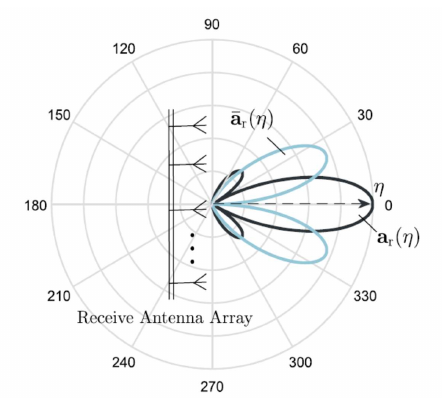
\includegraphics[width=0.6\linewidth]{figs/fig3.12}
%     \caption{Sum and difference beam patterns for monopulse ratio algorithm
%         \cite{Zhu2016}}
%     \label{fig:}
% \end{figure}

% Monopulse ratio is typically used to estimate a single AOA or resolvable angles
% (far spaced targets which are not located within the same beam). However, there
% are some modifications that use a complex monopulse ratio and allow one to
% detect the multiple targets in a certain beam and estimate their angle
% positions \cite{Luoshengbin2016} \cite{Sherman2011}.  


В \cite{Zhu2016} представлена ещё одна реализация метода моноимпульса, не требующая 
поиска нуля функции \eqref{eq:3.11}
\begin{equation}
    \label{eq:3.19}
    \zeta_n = \frac{p(\eta_n - \delta) - p(\eta_n + \delta)}{p(\eta_n - \delta)
        + p(\eta_n + \delta)} =
    \frac{\sin(\psi - \eta_n)\sin\delta}{1 - \cos(\psi - \eta_n)\cos \delta}
\end{equation}

\begin{equation}
    \label{eq:3.20}
    \psi = \eta_n - \arcsin(
    \zeta_n \frac{\sin\delta}{\sin^2 \delta + \zeta^2_n \cos^2\delta}
    -
    \frac{\zeta_n \sqrt{1-\zeta^2_n} \sin \delta \cos \delta}{\sin^2\delta +
        \zeta^2_n \cos^2 \delta}
    )
\end{equation}
где $\psi_n = 2\pi \frac{d}{\lambda} \sin \phi$ -- обобщенный угол 
главного лепестка с азимутальным направлением $\phi$,  $\eta$ -- центральный угол между двумя лучами моноимпульса, 
$n$ -- индекс лучшей пары лучей, $\delta = \frac{\pi}{N}$, $N$ -- число элементов в АР, $p(\eta)$ 
мощность сигнала, измеренной с луча, направленного на обобщенный угол $\eta$.

\begin{figure}[ht!]
    \centering
    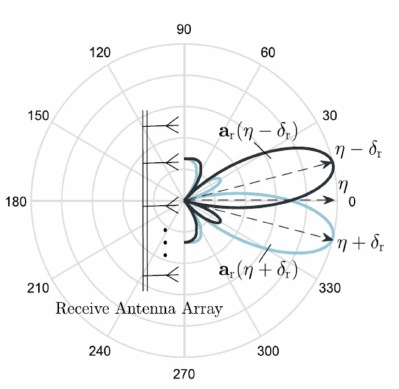
\includegraphics[width=0.45\linewidth]{figs/fig3.13}
    \caption{Сформированные лучи моноимпульса \cite{Zhu2016}}
    \label{fig:}
\end{figure}

Как показано в  \cite{Sherman2011},
этот метод может давать неправильный результат, если фактический AOA
находится вблизи максимума одной из двух сформированных ДН, а ОСШ достаточно низкое. 
В \cite{Sherman2011} для решения этой проблемы предлагается использовать ещё два дополнительных луча (см. рис. \ref{fig:3.14}).

\begin{figure}[ht!]
    \centering
    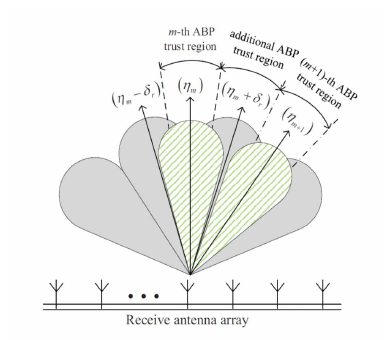
\includegraphics[width=0.6\linewidth]{figs/fig3.14}
    \caption{Метод монопульса с дополнительной парой лучей \cite{Tuncer2009}}
    \label{fig:3.14}
\end{figure}

\paragraph{Преимущества}%
\label{par:preimushchestva}

\begin{enumerate}
    \item На практике, этот метод более точный, чем методы Барлетта или Фурье, поскольку производная достаточно быстро изменяется вблизи AOA.
    \item Может быть реализован на фазированной антенной решетке с одним цифровым портом.
    \item Для оценки необходимо небольшое количество измерений. 
\end{enumerate}

\paragraph{Недостатки}%
\label{par:nedostatki}
\begin{enumerate}
    \item Поскольку является вариацией метода Фурье, его точность будет зависеть 
    от ширины главного лепестка ДН. Увеличение ОСШ или времени оценки не приведет к улучшению результата. 
    \item В случае двух близко расположенных источников сигнала, может наблюдаться значительная систематическая ошибка. 
\end{enumerate}

\subsubsection{Метод Кейпона}%
\label{sub:minimum_variance_distortionless_response_estimator_capon_method_}
\label{sec:Capon}

Другой алгоритм, основанный на методе Фурье -- Minimum Variance
Distortionless Response Estimator (MVDR), также называемый методом Кейпона \cite{Stoica2005,Allen2006, Godara2004}. 
Основная идея заключается в том, чтобы с помощью формирования ДН 
минимизировать мощность со всех направлений, при постоянном усилении для некоторого направления $\phi$.

\begin{figure}[h]
    \centering
    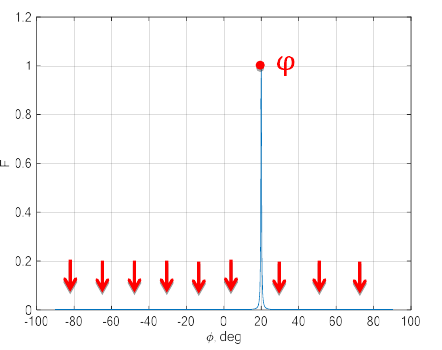
\includegraphics[width=0.6\linewidth]{figs/fig3.15.png}
    \caption{Основная идея метода Кейпона}
    \label{fig:3.15}
\end{figure}
Выбор весовой вектора в этом случае становится задачей нелинейного программирования 
\cite{Stoica2005, Godara2004}
\begin{equation}
    \label{eq:3.21}
    \vec w(\phi) = \frac{\hat{\vec M}^{-1} \vec s (\phi)}{\vec s^H(\phi)
        \hat{\vec M}^{-1} \vec s(\phi)},
\end{equation}
где $s(\phi)$ -- фазирующий вектор, определенный в \eqref{eq:3.2}, $\vec{\hat M}$ корреляционная матрица \eqref{eq:3.7}.
Искомая функция принимает следующий вид
\begin{equation}
    \label{eq:3.22}
    p(\phi) = \frac{1}{s^H(\phi) \vec M^{-1} \vec s(\phi)}
\end{equation}
Выражение \eqref{eq:3.22} представляет собой принятую мощность. Пики этой функции соответствуют найденными углам прихода. 
\paragraph{Преимущества}%
\begin{enumerate}
    \item Метод Кейпона обеспечивает высокую точность оценки AOA.
    \item Может быть использован для нахождения нескольких AOA, благодаря сверхразрешению. 
    \item Может быть реализован аппаратно, поскольку функция \eqref{eq:3.22} имеет смысл принятой мощности.
\end{enumerate}
\paragraph{Недостатки}%
\begin{enumerate}
    \item Разрешение ограничено, даже если корреляционная матрица $\vec M$
    известна точно. Для улучшения разрешения необходимо увеличивать ОСШ или
    количество элементов АР
    \item Нахождение обратной матрицы, которое необходимо для этого метода, требует больших вычислительных затрат.
\end{enumerate}